\documentclass[10pt, a4paper]{report}
\usepackage[utf8]{inputenc}
\usepackage[T1]{fontenc}
\usepackage{amsmath}
\usepackage{amsfonts}
\usepackage{amssymb}
\usepackage{graphicx}
\usepackage{hyperref}
\hypersetup{
	colorlinks=true,
	linkcolor=blue,
	filecolor=magenta,      
	urlcolor=cyan,
}
\author{Pranav Gade\thanks{notes from lectures by Prof. Bibek Singh}}
\date{Dec. 2020 - Mar. 2020}
\title{System Management}


\begin{document}
	\maketitle
	\tableofcontents
		\section*{Links}
	\begin{itemize}
		\item Email: \href{mailto:bibek@iiitl.ac.in}{bibek@iiitl.ac.in}
		\item Shared drive: \href{https://drive.google.com/drive/folders/0AP18u-62wQ93Uk9PVA}{https://drive.google.com/drive/folders/0AP18u-62wQ93Uk9PVA}
		\item Phone number: 6392333966
	\end{itemize}
	\newpage
	\setcounter{chapter}{-1}
	\chapter{Introduction}
	\section*{Sample assignment}
	\subsection*{Bank wants user to maintain a minimum balance of Rs. 1000 all the time.}
	Algorithm:
	\begin{enumerate}
		\item Have a variable $ x $
		\item $ x = 1000 $
		\item $ if(balance < x) $ then DO NOT ALLOW TRANSFER
		\item Display error message to user
	\end{enumerate}
	\section*{History of Computers}
	\href{https://docs.google.com/document/d/1AKiCZ0Cal-O2vfzAeWJqINXd06CINqywDTrg5B8KlEw/edit?usp=sharing}{Reading Assignment 1: History of Computers}
	\chapter{Computer Fundamentals}
		\section{Evolution of computers}
			Computers started as very large machines, taking up massive amounts of energy. They used terminals as input, and printers as output.
			
			Scientists used computers for simulations, solving, and regression analysis. Until 1993, non-structured languages like COBOL, Pascal, etc. were available. Around 1993, structured languages like C appeared. And around 1998, Object Oriented languages started appearing. These focused on layered/tiered approach. Around the same time, layered approach to server design became popular.
			\\ \\
			\begin{tabular}{|p{0.45\linewidth} | p{0.45\linewidth}|}
				\hline
				Non-Structured Languages & Structured Languages \\
				\hline
				Allowed goto/jump statements, so you could jump to any line of code. & Excecution proceeds sequentially \\
				\hline
				This made stuff very convoluted & This makes the program easier to follow \\
				\hline
			\end{tabular}
			\\ \\
			Layered approach in server design(fig. \ref{fig:request-response-model}) provides encapsulation. This allows a more granular control over security and permission management. It also helps to mitigate downtimes and service issues. Along with this, multiple services can interact with, say, the same database server, thus reducing redundancy.
			\begin{figure}
				\centering
				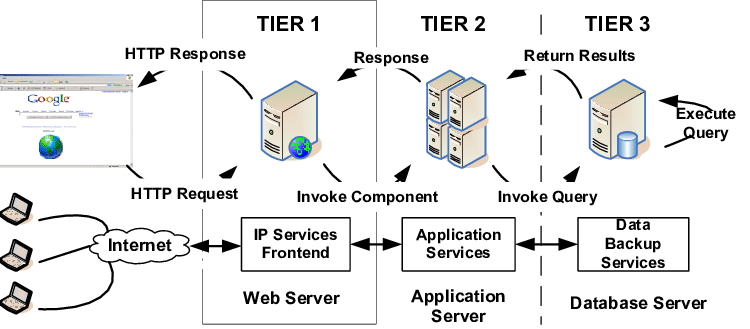
\includegraphics[width=0.7\linewidth]{img/request-response-model}
				\caption[Request - Response Model]{\textbf{Request - Response Model}: User interacts with the Web server; Business logic is in Application server; User data is stored in Database server}
				\label{fig:request-response-model}
			\end{figure}
		\section{Software requirements}
			\begin{itemize}
				\item \textbf{Functional Requirements:} This describes how the software must function/operate.
				\item \textbf{Non-Functional Requirements:} These are factors like performance, load, number of users, etc.
			\end{itemize}
%	\chapter{Basics of OS and Memory management}
	\chapter{Introduction to Networking}
	\section{What is a network}
	\begin{itemize}
		\item A set of devices (often referred to as nodes) connected by communication links.
		\item An interconnected(physically or logically) collection of autonomous computers. \\
		Two computers are said to be interconnected if they can exchange information. The connection may be copper wire, infra-red, microwave, fiber optics, satellite, etc.
	\end{itemize}
	\subsection{The Internet} is a computer network that interconnects hundreds of millions of computing devices throughout the world.\\
	$\star$Client - a device that can make a request on a network.\\
	$\star$Server - a device that can respond to the request.\\
	These systems are called hosts.
	\subsubsection{ISP} a collection of network routers/switches. 
%	\chapter{Use of Computer in Commerce}
\end{document}